\documentclass[aspectratio=169]{beamer}

\usepackage[utf8]{inputenc}
\usepackage[T1]{fontenc}
\usepackage[english]{babel}
\usepackage{graphicx}
\usepackage{amsmath,amssymb}
\usepackage{tikz}
\usepackage{tabularx}
\usepackage{booktabs}

% --- PWr color scheme (same as CtF/SOCO templates) ---
\xdefinecolor{pwrone}{rgb}{0.6015625,0.203125,0.17578125}
\xdefinecolor{pwrtwo}{rgb}{0.94140625,0.81640625,0.6328125}
\mode<presentation>
{
    \usetheme{Warsaw}
    \setbeamercolor{structure}{fg=pwrone}
    \setbeamercolor*{palette primary}{use=structure,fg=pwrtwo,bg=pwrone}
    \setbeamercolor*{palette quaternary}{use=structure,fg=pwrone,bg=pwrtwo}
}
\usetheme{Warsaw}

% --- Frame counter in footer ---
\newcommand*\oldmacro{}
\let\oldmacro\insertshortauthor
\renewcommand*\insertshortauthor{%
    \leftskip=.3cm%
    \insertframenumber\,/\,\inserttotalframenumber\hfill\oldmacro%
}

\newcolumntype{C}{>{\centering\arraybackslash}X}

\title[Fibonacci Neighborhood for PFSP]
{Hybrid Neighborhood Evaluation\\
with focus on the Fibonacci-distance Neighborhood\\
for the Permutation Flow Shop Problem}
\author[R.~Wojew\'odzki, W.~Bo\.zejko]
{Remigiusz Wojew\'odzki \and Wojciech Bo\.zejko}
\institute{
{\tt remigiusz.wojewodzki@gmail.com} \quad {\tt wojciech.bozejko@pwr.edu.pl}\\[1mm]

\includegraphics[height=8mm]{logo_PWR.png}
}
\date{ICAISC 2026\vspace{8mm}}

\begin{document}

% ===== SLIDE 1: TITLE =====
\frame{\thispagestyle{empty}\titlepage}

% ===== SLIDE 2: OUTLINE =====
\begin{frame}{Outline}
    \tableofcontents
\end{frame}

% ===== SLIDE 3 =====
\section{Introduction}
\begin{frame}{Introduction}
    \begin{itemize}
        \item \textbf{Permutation Flow Shop Problem (PFSP):} NP-hard for $m \geq 3$. Neighborhood choice drives metaheuristic quality.
        \item Classical neighborhoods trade off coverage and cost:
            \begin{itemize}
                \item \textbf{Adjacent swap:} $n{-}1$ moves, only short-range.
                \item \textbf{Dynasearch:} $O(n^2)$ candidates, expensive per call.
                \item \textbf{Motzkin arcs:} structured but $O(n^3)$ DP --- breaks beyond $n \sim 100$.
            \end{itemize}
        \item \textbf{Fibonacci-distance insertion:} $O(n \log n)$ moves spanning short \emph{and} long range. Stays tractable up to $n = 500$ and beyond.
        \item This talk: define the Fibonacci neighborhood, position it among the other elementary moves, and show its role within hybrid local search (TS, SA).
    \end{itemize}
\end{frame}

% ===== SLIDE 4 =====
\section{Fibonacci Neighborhood}
\begin{frame}{The Fibonacci-distance Neighborhood}
    \textbf{Definition.} Given $\pi = (\pi_0, \dots, \pi_{n-1})$, define moves
    \[
        N_{\mathrm{fib}}(\pi) \;=\; \bigl\{\, \mathrm{insert}(\pi_i \to i + F_k) \;:\; 0 \leq i < n,\ F_k \leq n - i \,\bigr\},
    \]
    where $F_k = 1, 2, 3, 5, 8, 13, 21, \dots$ are Fibonacci numbers.

    \textbf{Size:} $|N_{\mathrm{fib}}(\pi)| = O(n \log n)$. Local + long-range coverage from a single rule.

    \vspace{0.2cm}
    \textbf{Idea.} A geometric, golden-ratio-scaled set of move distances from position $i$:
    \begin{center}
    \begin{tikzpicture}[scale=0.75]
        \foreach \x in {0,1,2,...,12} \fill (\x,0) circle (2pt);
        \node[below=2pt] at (0,0) {\small$i$};
        \draw[thick,pwrone,->] (0,0.1) to[bend left=35] (1,0.1); \node[pwrone] at (0.5,0.45) {\tiny$F_1$};
        \draw[thick,pwrone,->] (0,0.1) to[bend left=40] (2,0.1); \node[pwrone] at (1.0,0.7) {\tiny$F_2$};
        \draw[thick,pwrone,->] (0,0.1) to[bend left=45] (3,0.1); \node[pwrone] at (1.5,1.0) {\tiny$F_3$};
        \draw[thick,pwrone,->] (0,0.1) to[bend left=50] (5,0.1); \node[pwrone] at (2.5,1.4) {\tiny$F_4$};
        \draw[thick,pwrone,->] (0,0.1) to[bend left=55] (8,0.1); \node[pwrone] at (4.0,1.9) {\tiny$F_5$};
    \end{tikzpicture}
    \end{center}
\end{frame}

% ===== SLIDE 5 =====
\begin{frame}{Why Fibonacci? --- Properties}
    \begin{itemize}
        \item \textbf{Golden-ratio scaling.} Consecutive jump distances grow by $\varphi \approx 1.618$ --- the densest non-uniform integer sequence avoiding any short cycle.
        \item \textbf{Logarithmic per-position.} Only $O(\log n)$ jump lengths per starting position; total $O(n \log n)$ moves \emph{vs.} $O(n^2)$ for full insertion or dynasearch.
        \item \textbf{Tridiagonal QUBO.} The QUBO matrix has bandwidth 2 --- embeds natively on D-Wave with no chain breaks. Scales cleanly to $n = 500$.
        \item \textbf{Self-similarity.} Fibonacci shifts within a Fibonacci shift form a sub-neighborhood --- the move structure is recursive, well-suited to multi-scale local search.
    \end{itemize}
\end{frame}

% ===== SLIDE 6 =====
\section{Fibonacci in Hybrid Local Search}
\begin{frame}{Role in Hybrid Strategies}
    Four elementary neighborhoods are combined under five strategies (FC, PW, PA, BK, DP). Fibonacci's job in each:
    \begin{itemize}
        \item \textbf{FC --- Fixed Cycle:} Fibonacci breaks adjacent-swap stagnation between two dynasearch passes.
        \item \textbf{PA --- Performance-Adaptive:} the EMA-driven selector picks Fibonacci most often in mid-search, once adjacent saturates but before dynasearch becomes affordable.
        \item \textbf{BK --- Best-of-$K$:} Fibonacci is the cheapest non-trivial neighborhood to evaluate, so its candidates effectively come for free in the BK sweep.
        \item \textbf{Large $n$:} for $n \geq 200$ Fibonacci is the only elementary neighborhood that completes \emph{multiple} iterations within the time budget --- the rest degenerate to a single call.
    \end{itemize}
\end{frame}

% ===== SLIDE 7 =====
\section{Experiments}
\begin{frame}{Experimental Setup}
    \begin{itemize}
        \item \textbf{Benchmarks:} Taillard instances, $n \in \{20, 50, 100, 200, 500\}$, $m \in \{5, 10, 20\}$, 10 instances each, 5 seeds.
        \item \textbf{Time limits:} $t_{\max} \in \{0.1, 0.5, 1, 2, 5, 10\}$~s; metric: mean RPD to lower bound.
        \item \textbf{Algorithms:} Iterated Local Search (tabu $\tau{=}10$, MushroomList $k{=}10$); Simulated Annealing ($T_0{=}1000$, $\alpha{=}0.99$, reheat-kick on stagnation).
        \item \textbf{Quantum:} D-Wave Advantage 4.1, $5{,}000$ reads, windowed decomposition for $n > 19$.
        \item \textbf{Compared neighborhoods:} Adjacent, \textbf{Fibonacci}, Dynasearch, Motzkin.
    \end{itemize}
\end{frame}

% ===== SLIDE 8 =====
\begin{frame}{Scaling Behavior --- RPD vs.\ $n$}
    \begin{columns}
        \begin{column}{.55\textwidth}
            \centering
            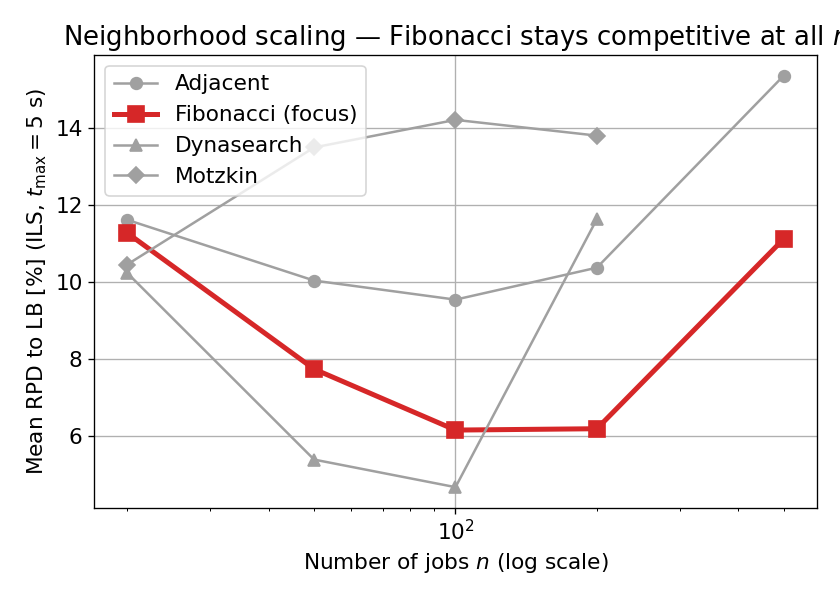
\includegraphics[width=\linewidth]{img/fib_scaling.png}
        \end{column}
        \begin{column}{.45\textwidth}\small
            \textbf{Observations} (ILS, $t_{\max}=5$\,s, $m{=}10$):
            \begin{itemize}
                \item Up to $n \approx 100$: Dynasearch wins, Fibonacci second.
                \item $n = 200$: Fibonacci \textbf{overtakes} Dynasearch (6.19\,\% vs.\ 11.63\,\%).
                \item $n = 500$: Dynasearch and Motzkin become intractable; Fibonacci continues at \textbf{11.12\,\%} --- the only classical neighborhood that still scales.
            \end{itemize}
        \end{column}
    \end{columns}
\end{frame}

% ===== SLIDE 9 =====
\begin{frame}{Gap vs.\ Time Limit --- Fibonacci within the Hybrid Pool}
    \begin{columns}
        \begin{column}{.5\textwidth}
            \centering
            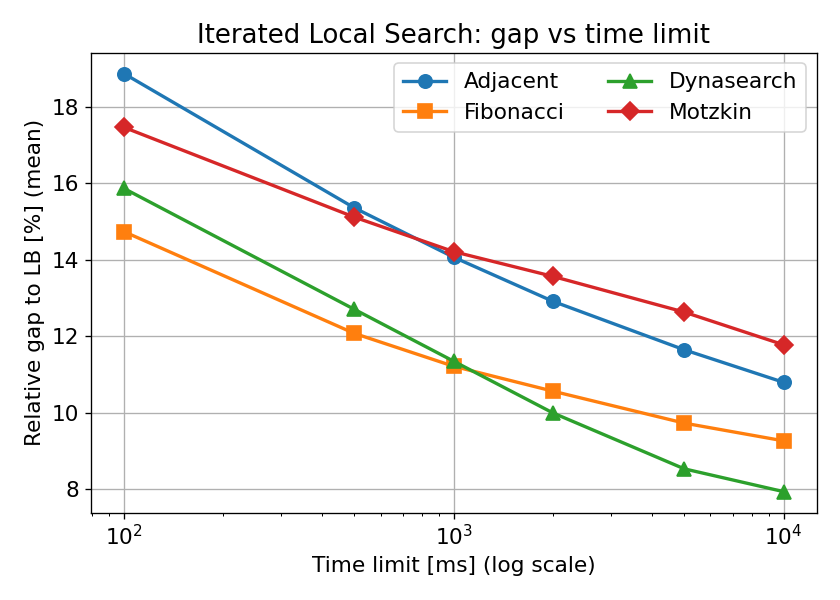
\includegraphics[width=\linewidth]{img/ils_gap.png}\\\small ILS
        \end{column}
        \begin{column}{.5\textwidth}
            \centering
            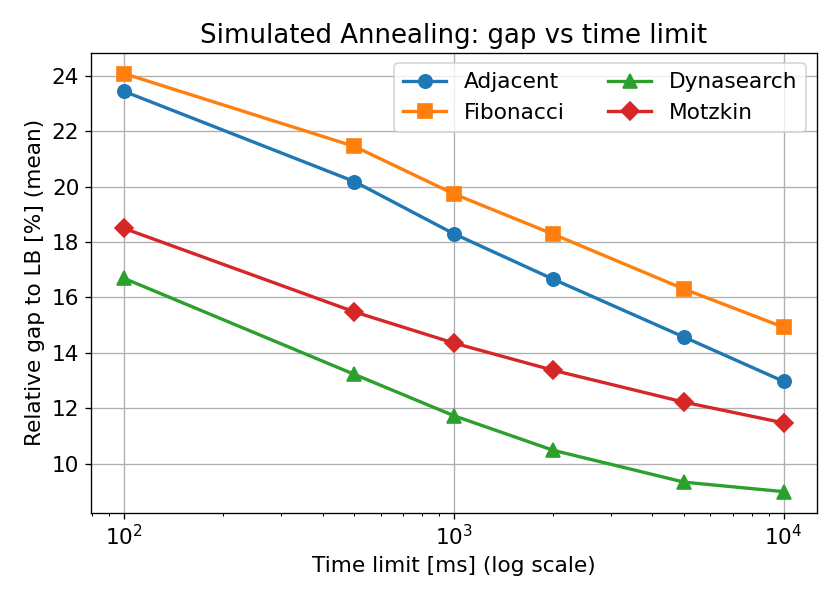
\includegraphics[width=\linewidth]{img/sa_gap.png}\\\small SA
        \end{column}
    \end{columns}

    \vspace{0.2cm}
    \begin{itemize}
        \item Fibonacci converges \textbf{fastest} (flat curve from $t_{\max} = 100$~ms onward) but plateaus highest --- ideal as the \emph{warm-up} neighborhood within a hybrid.
        \item Combined with a slower, deeper neighborhood (Motzkin or Dynasearch), Fibonacci's early-budget gain compounds with the later-budget refinement.
    \end{itemize}
\end{frame}

% ===== SLIDE 10 =====
\section{Conclusion}
\begin{frame}{Conclusion and Future Work}
    \textbf{Summary:}
    \begin{itemize}
        \item Fibonacci is the only elementary neighborhood that stays tractable from $n = 20$ to $n = 500$.
        \item Tridiagonal QUBO structure makes it the natural classical baseline for D-Wave QPU comparison.
        \item Inside a hybrid strategy (PA, BK), Fibonacci absorbs the early time budget cheaply; heavier neighborhoods then refine.
        \item Empirically, Fibonacci wins outright above $n = 200$ where its rivals run out of computational budget.
    \end{itemize}

    \vspace{0.2cm}
    \textbf{Future work:}
    \begin{itemize}
        \item Quantum-assisted Fibonacci neighborhood (windowed QUBO, $n$ up to $500$).
        \item Multi-armed bandit selection over neighborhoods with Fibonacci as the low-cost arm.
        \item Hybrid generalization: Fibonacci-of-Fibonacci composite moves.
    \end{itemize}
\end{frame}

\end{document}
